\subsection{Гистограммы}
\begin{itemize}
	\begin{figure}[H]
		\begin{tabular}{ccc}
			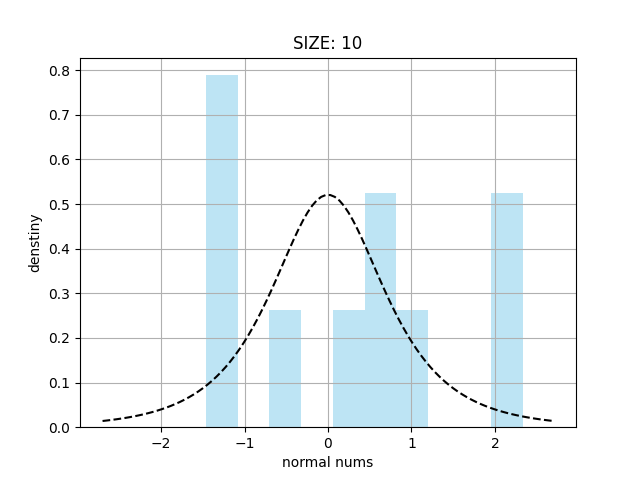
\includegraphics[scale=0.333]{task_1/resource/normal10.png}
			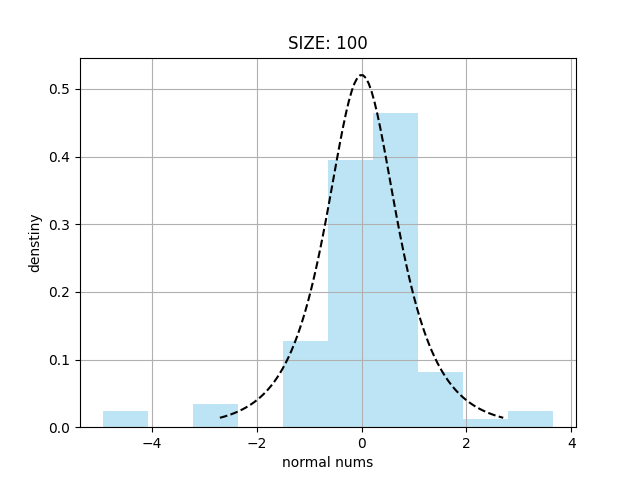
\includegraphics[scale=0.333]{task_1/resource/normal100.png}
			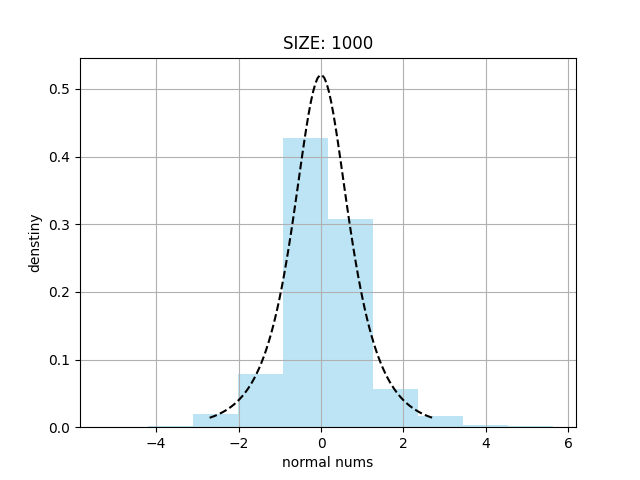
\includegraphics[scale=0.333]{task_1/resource/normal1000.png}
		\end{tabular}
		\caption{Гистограмма и плотность вероятности для нормального распределения [N = 10, 100, 1000]} 
	\end{figure}
	
	\begin{figure}[H]
		\begin{tabular}{ccc}
			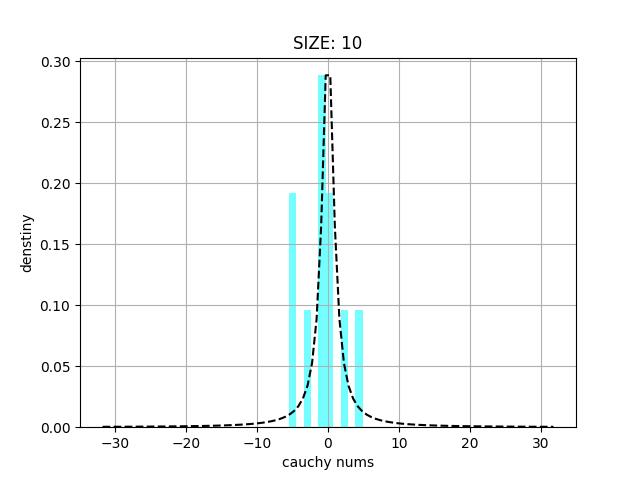
\includegraphics[scale=0.333]{task_1/resource/cauchy10.png}
			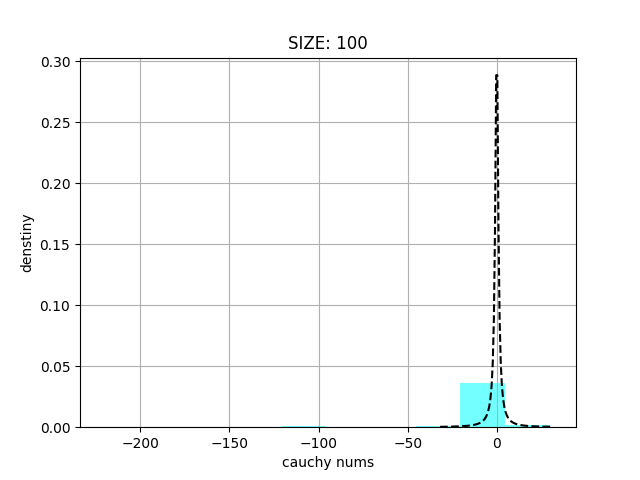
\includegraphics[scale=0.333]{task_1/resource/cauchy100.png}
			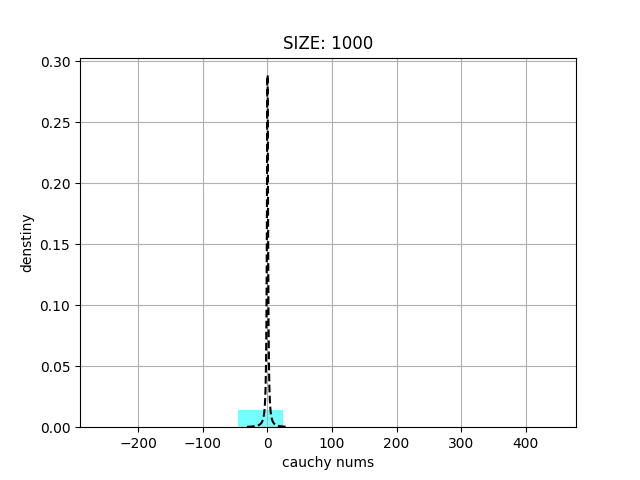
\includegraphics[scale=0.333]{task_1/resource/cauchy1000.png}
		\end{tabular}
		\caption{Гистограмма и плотность вероятности для распределения Коши [N = 10, 100, 1000]}
	\end{figure}
		
	\begin{figure}[H]
		\begin{tabular}{ccc}
			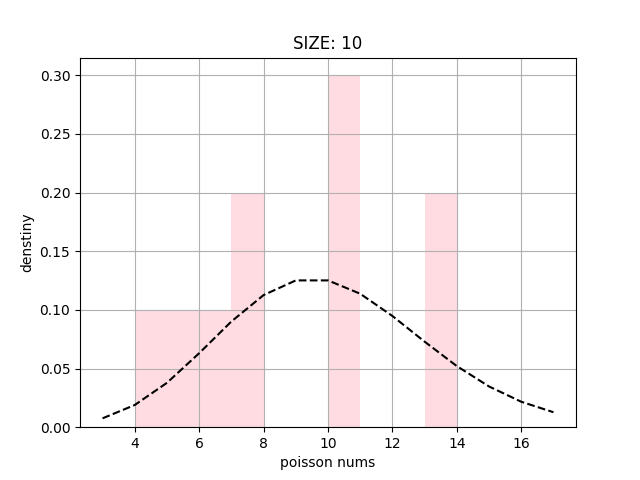
\includegraphics[scale=0.333]{task_1/resource/poisson10.png}
			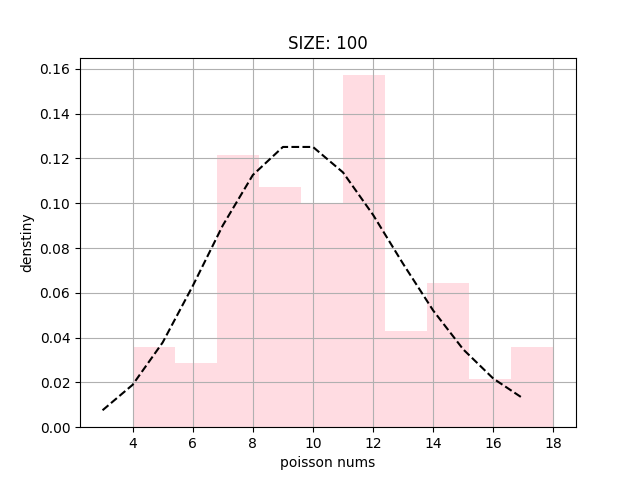
\includegraphics[scale=0.333]{task_1/resource/poisson100.png}
			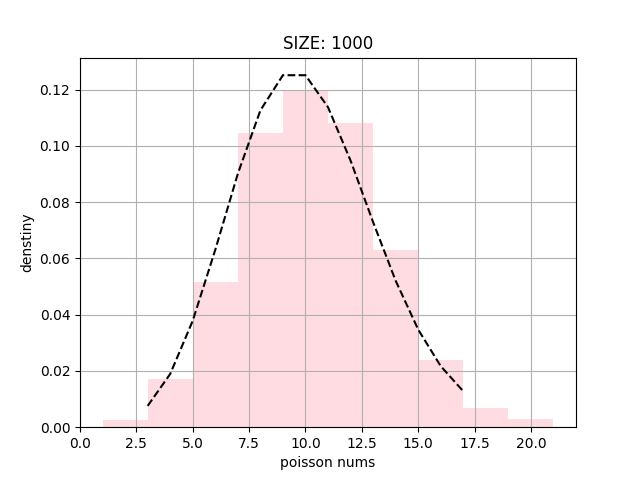
\includegraphics[scale=0.333]{task_1/resource/poisson1000.png}
		\end{tabular}
		\caption{Гистограмма и плотность вероятности для распределения Пуассона [N = 10, 100, 1000]} 
	\end{figure}
	
	\begin{figure}[H]
		\begin{tabular}{ccc}
			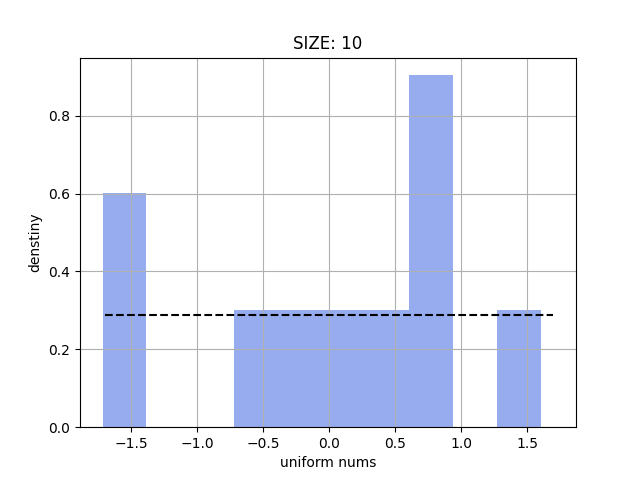
\includegraphics[scale=0.333]{task_1/resource/uniform10.png}
			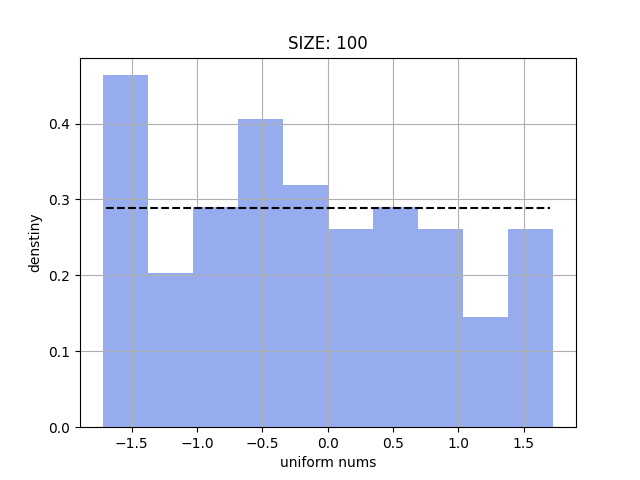
\includegraphics[scale=0.333]{task_1/resource/uniform100.png}
			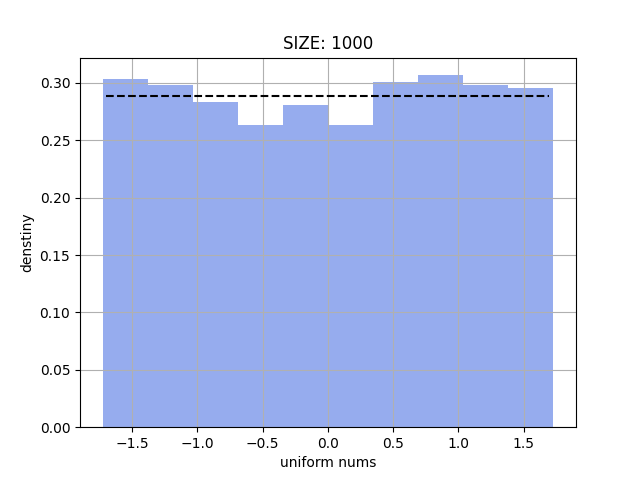
\includegraphics[scale=0.333]{task_1/resource/uniform1000.png}
		\end{tabular}
		\caption{Гистограмма и плотность вероятности для равномерного распределения [N = 10, 100, 1000]} 
	\end{figure}

\end{itemize}